\chapter{Methodology}
\label{chap:methodology}

 
 
 \section{Project description}
 
 \begin{itemize}
  	\item Papiit
 	\item Temixco
 	\item Grafica de radiación
 	\item Hay potencial
 	\item cafetería modeling
 	\item aspersores, direct evaporative modelling, foto del osm
 \end{itemize}
 

This thesis work is a product of the Papiit project, Estudio teórico-experimental del enfriamiento evaporativo en eficicaciones.
Objetivo de Papiit. 

This project study and aim to simulate the evaporative cooling process that takes place in the sprayers located within the IER cafeteria area. As the IER is situated in Temixco, a township of the state of Morelos, the numerical experiments were carried out with local data.

 Temixco is a city located in the mexican state of Morelos, it borders with Cuernavaca and Jiutepec. It has a latitud of 18.85°, -99.22° of longitud, 1253 MSL and 89,869 $km^{2}$ of territorial extension. According to the population and housing census made in 2020 by the Instituto Nacional de Estadística, Geografía e Informática (INEGI)[1]the city has a population of 122,263 people. Its climate is form by to kinds; warm sub-humid and semi-warm sub-humid climate [2]. The temperature range is 18-24°C and the precipitation range, which most is in summer, is 800-1200 mm. 
 
\begin{figure}
 \centering
 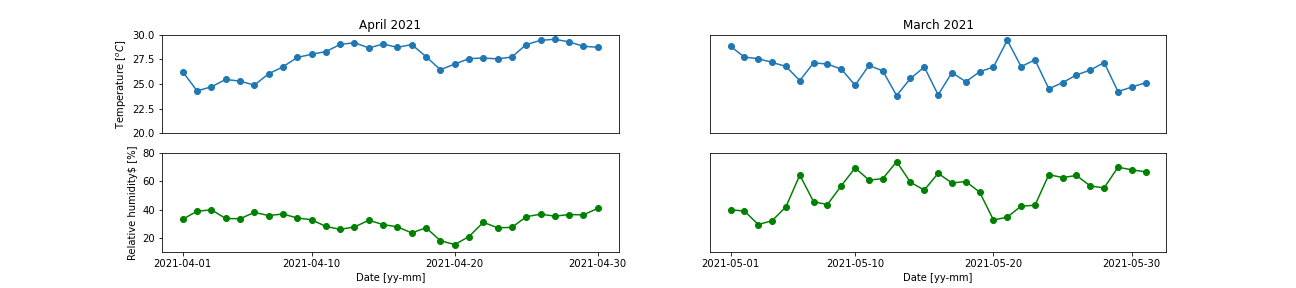
\includegraphics[scale=0.3]{tempVShum}
 \caption{	
 Mean temperature and relative humidity in March and April 2021 according to ESOLMET.
 \label{fig:tempvshum}
 }
\end{figure}

\begin{figure}
 \centering
 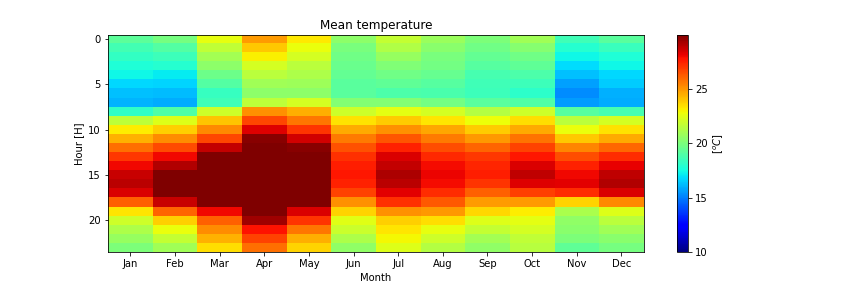
\includegraphics[scale=0.4]{Temperature}
 \caption{	
 Temperature, IER 2021 according to ESOLMET.
 \label{fig:temp}
 }
\end{figure}

\begin{figure}
 \centering
 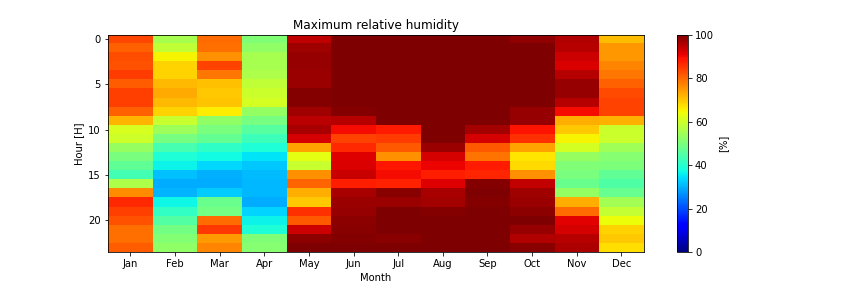
\includegraphics[scale=0.4]{relhum}
 \caption{	
 Relative humidity, IER 2021 according to ESOLMET.
 \label{fig:rh}
 }
\end{figure}


\begin{figure}
 \centering
 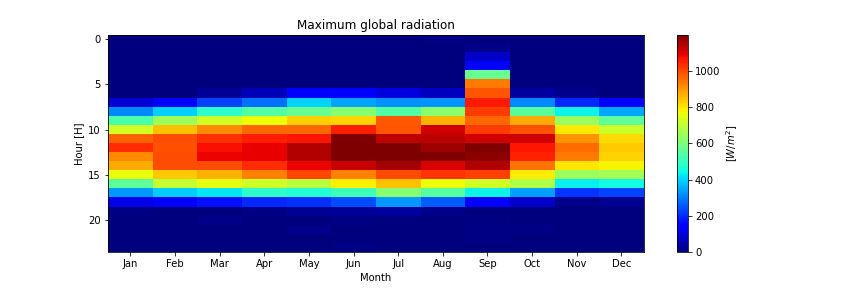
\includegraphics[scale=0.4]{Ig}
 \caption{	
 Global radiation, IER 2021 according to ESOLMET.
 \label{fig:Ig}
 }
\end{figure}



The zone where this effect is been studying is the cafeteria area of the IER. It corresponds the second floor of a building north-south oriented. 

\begin{figure}
 \centering
 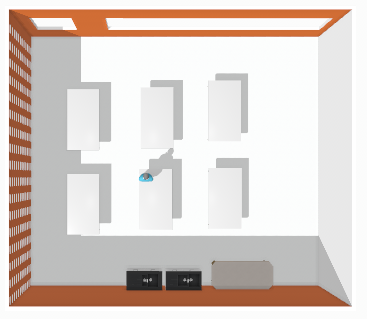
\includegraphics[scale=1]{cafeteria3D}
 \caption{	
 IER cafeteria
 \label{fig:3D}
 }
\end{figure}

\begin{figure}
 \centering
 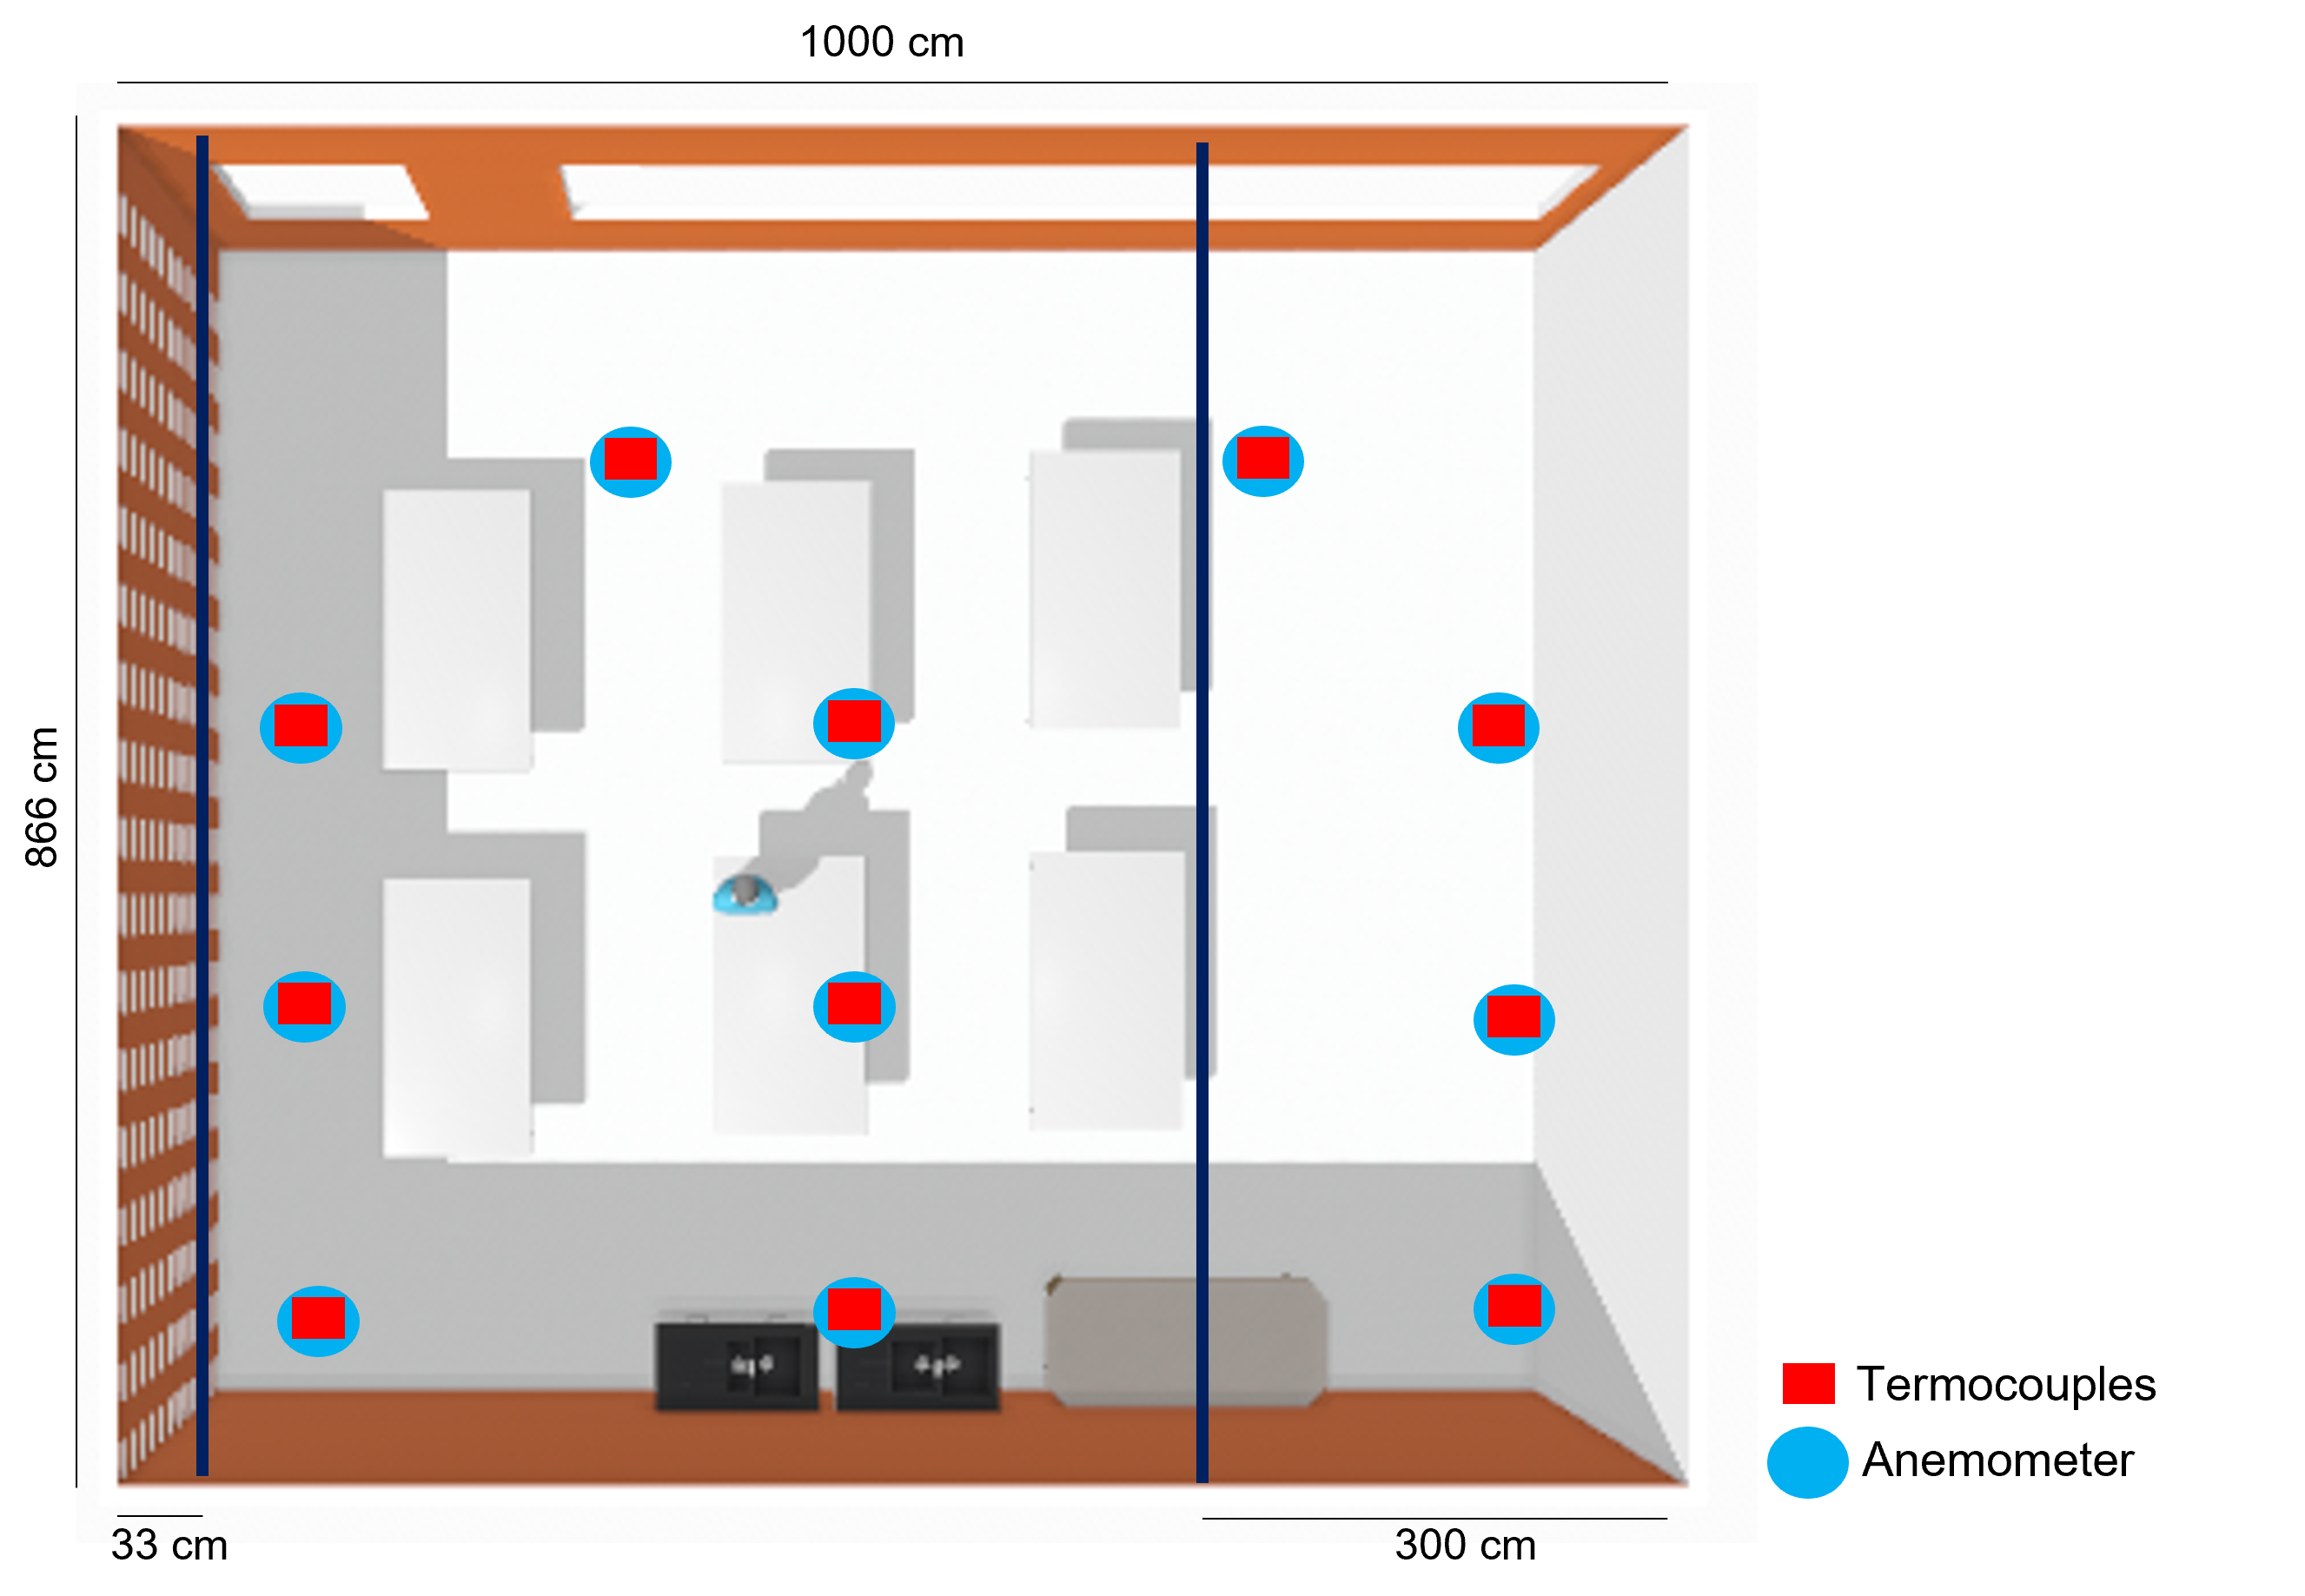
\includegraphics[scale=0.5]{cafeteria_sensores}
 \caption{	
 IER cafeteria
 \label{fig:sensores}
 }
\end{figure}







 
 
 \section{Numerical experiments}
 
 Hay que esperar un poco, pero podría ser numerical simulation and validation… pero ya que tengamos más información lo consideramos.


También hay que considerar si habrá algunos apéndices, reportando tus libretas, me parece interesante documentar tu proceso de aprendizaje.
 
 \section{Validation process}
 
